% 1986 年上海卷理工农医类第 6 题：抛物线与圆
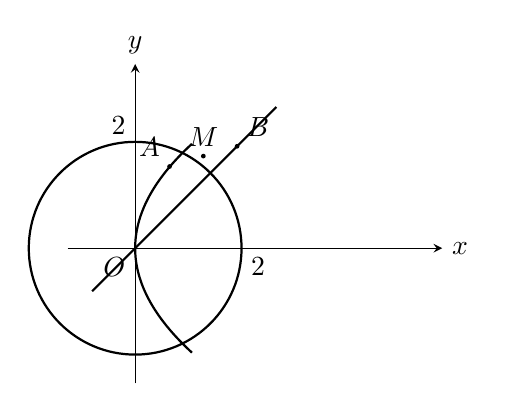
\begin{tikzpicture}[scale=0.78,>=stealth]
  \draw[->] (-1.1,0)--(5.0,0) node[right] {$x$};
  \draw[->] (0,-2.2)--(0,3.0) node[above] {$y$};
  \draw[thick] (0,0) circle (1.732);
  \draw[thick,domain=-1.7:1.7,samples=100]
    plot ({0.32*\x*\x},{\x});
  \draw[thick] (-0.7,-0.7)--(2.3,2.3);
  \fill (0.56,1.33) circle (1.1pt) node[above left] {$A$};
  \fill (1.66,1.66) circle (1.1pt) node[above right] {$B$};
  \fill (1.11,1.50) circle (1.1pt) node[above] {$M$};
  \node[below left] at (0,0) {$O$};
  \node[below] at (2,0) {$2$};
  \node[left] at (0,2) {$2$};
\end{tikzpicture}
